\clearpage
\section{Correct-clock TDC repeat: 14 November 2026}
Board \texttt{PM12-K7-3A17A1B402212223}; MCU1803.
Current SRAM diagnostic: \texttt{c7531465}. TDC channels9--12 pass the
corrected-clock repeat. Earlier measurements remain historical observations.

\subsection{Clock correction and procedure}
The audited MCLK is40.0787MHz, rather than the previously assumed120MHz.
The TDC MMCM input divider was changed from3 to1, retaining multiplier30
and output dividers2/2/4: VCO1202.361MHz, fast601.1805MHz and
coarse300.59025MHz. Corresponding MCLK and TDC-reference constraints were
corrected. No external PLL, MCU, CPLD or nonvolatile image was changed.
Implementation WNS is0.085ns and WHS0.066ns; no DRC errors or critical warnings.

For each channel: quiet window,16-event discovery, count tests1/64/512/1024,
25 serializer positions with128 events each, then another quiet window.
All128 captures were read back as raw13-bit words and independently checked.
All19,268 events were conserved; eight quiet windows were empty and there
were no cross-channel records. Capture generations were consecutive.

\begin{center}
\begin{tabular}{rrrr}\toprule
Channel & Fine slope [codes/ns] & Coarse gain [codes/bin] & Result\\\midrule
9 & -46.196 & 1.25231 & PASS\\
10 & -46.164 & 1.25160 & PASS\\
11 & -46.160 & 1.25111 & PASS\\
12 & -46.184 & 1.24769 & PASS\\\bottomrule
\end{tabular}
\end{center}
The predicted coarse gain is1.25. Fine slopes are relative raw-code responses,
not calibrated TDC bin sizes or intrinsic jitter measurements. Coarse values
are unwrapped across their empty arc and folded modulo10, one Kasli word,
to remove whole-word start branches; this does not establish absolute LHC
trigger alignment.

\subsection{Regression and remaining findings}
Digital ADC acquisition passed on all12 channels and both banks using
physical and bit-exact synthetic captures. This is not new analog qualification.
HDMI/SPI signatures were correct, but8 of12 reads restarted the SYS counter;
that separate fault remains open. Kasli slot6 SPI outputs remained driven.
The CFD11 MUX7 divider finding also remains open. USB stimulus remains on10.
Channels1--8 TDC require their own stimulated repeat.
The historical campaign coverage table is unchanged; these are a separate,
versioned qualification series, not retroactive edits to its source contract.
Raw data, source snapshots, bitstream, validation and hashes are retained in
\texttt{tdc\_live120/evidence-clock40-20261114}.
\clearpage
\begin{figure}[p]\centering
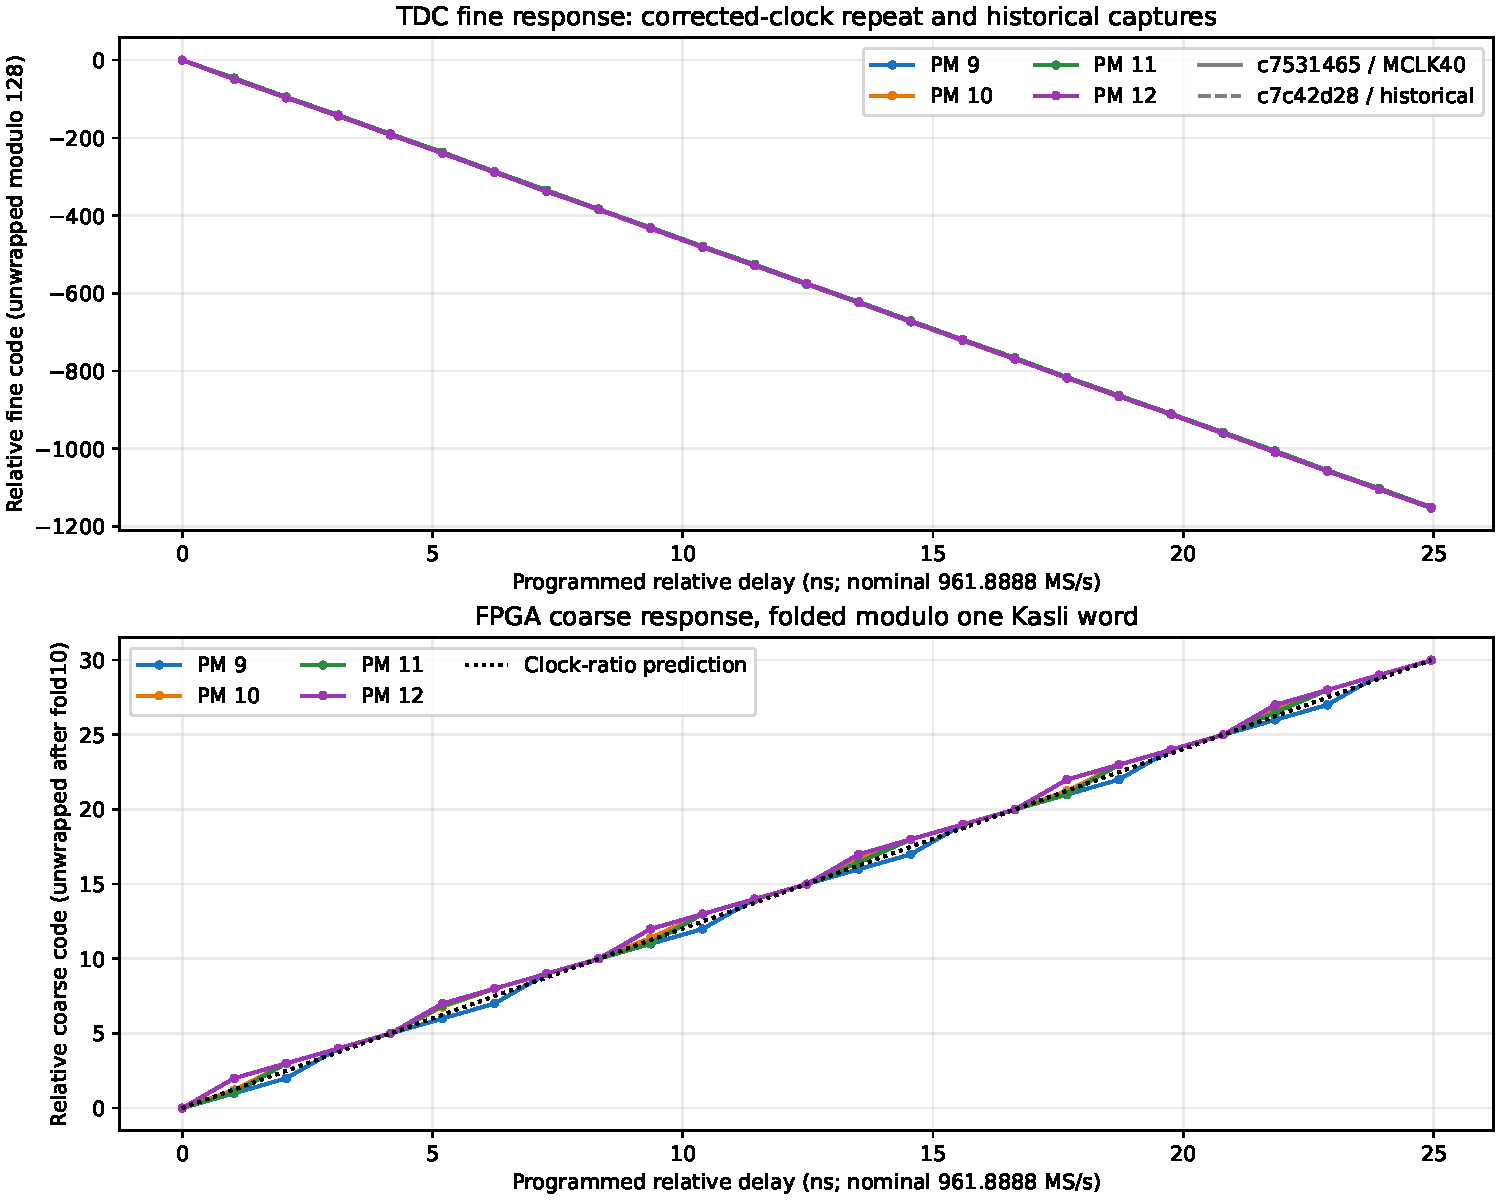
\includegraphics[width=\textwidth,height=.88\textheight,keepaspectratio]{tdc-clock40-phase.pdf}
\caption{Correct-clock relative fine and coarse response; all four channels overlaid.}
\end{figure}
\clearpage
